\section{Algoritmo exacto para la resoluci\'on de CACM}

\subsection{Notaci\'on} \label{exacto:notacion}

\begin{itemize}
	\item $G$ $=$ Grafo al que se le quiere encontrar el \emph{CACM}
	\item $P$ $=$ El camino a encontrar
	\item $v, w$ $=$ Los nodos de origen y destino del camino $P$ a encontrar
	\item $K$ $=$ Cota superior del peso $\omega_1$ del camino $P$ a encontrar
\end{itemize}

\subsection{Explicaci\'on detallada del algoritmo propuesto} \label{exacto:explicacion}

\subsubsection{Descripci\'on}

El algoritmo que se propone para encontrar la soluci\'on exacta al poblema del \emph{CACM}, consiste en encontrar todos los caminos simples de $v$ a $w$
y encontrar el camino $P$ que tenga el menor peso $\omega_2$ pero que $\omega_1$ no supere a $K$.

Se va a realizar un backtracking que s\'olo chequee los caminos que no superen a $K$ el peso de $\omega_1$, y que descarte los caminos en cuanto
detecta que no puede mejorar una soluci\'on que ya tenga almacenada como candidato a ser la de menor peso $\omega_2$.

El algoritmo ser\'a una funci\'on recursiva, pas\'andole como argumentos el grafo, los nodos de origen ($u$ el cual en la primer llamada va a ser $v$,
el nodo origen del problema) y destino ($w$), el limite K, y un camino encontrado hasta el momento, que va desde el nodo de origen del problema ($v$), al nodo de orgen pasado a la funci\'on ($u$).

En cada llamada recursiva, la funci\'on recorre todos los adyacentes a $u$, y por cada uno (nombremoslo $z$) llama recursivamente quitando el eje $(u,z)$ al grafo,
,indic\'andole como nodo de origen a $z$, y agregando al camino encontrado hasta el momento el nodo $z$. Luego se queda con el mejor camino que encontr\'o entre cada uno de los adyacentes.

A su vez, antes de comenzar con todas las llamadas recursivas, se ejecuta \emph{Dijkstra} desde el nodo $u$ sobre los pesos $\omega_1$. Si la peso $\omega_1$ del camino m\'inimo desde $u$ a $w$ tiene un valor mayor a $K$, entonces se retorna que no hay soluci\'on sin comenzar con la recursi\'on, ya que los caminos que hubiesenn, va a tener un peso $\omega_1$ mayor a $K$ (ya que el m\'inimo es mayor a $K$)

Se agrega tambi\'en antes de comenzar con la recursi\'on, se obtienen los caminos m\'inimos (tanto de $\omega_1$ como de $\omega_2$) desde el nodo de destino $w$ al resto del grafo.
Estando dentro de las llamadas recursivas, s\'olo avanza al siguiente nodo si el camino m\'inimo desde dicho nodo hacia $w$ cumple con la cota de $K$ en $\omega_1$ y que sea mejor en peso $\omega_2$ que el mejor camino ya calculado (como no son dirigidos los grafos, es igual al camino desde $w$ a ese nodo).

\subsubsection{Algoritmo}

\begin{algorithm}[!h]
\caption{cacm\_exacto} \label{exacto:pseudo}
\end{algorithm}
\begin{algorithmic}[1]
	\Require \emph{grafo}: el grafo al cual se tiene que encontrar el \emph{CACM}
	\Require \emph{u}: el nodo de origen
	\Require \emph{w}: el nodo de destino
	\Require \emph{K}: cota del peso $\omega_1$
	\Require \emph{solucion}: posible soluci\'on que se tiene hasta el momento. Por aca se recibe un camino posible y se actualiza en cada llamada recursiva con el mejor camino encontrado. Cuando terminen todas las llamadas recursivas, se retorna por aca el \emph{CACM} encontrado. En la primera llamada se debe llamar con una soluci\'on que s\'olo contenga al nodo de partida $v$.
	\Statex
	\Ensure Retorna $verdarero$ si encontr\'o un camino de $u$ a $w$, $falso$ si no encontr\'o camino.
	\Statex
	\State solucion\_mejor $\gets$ $[]$
	\Statex
	\Procedure{cacm\_exacto}{$Grafo$: grafo, $Nodo$: u, $Nodo$: w, $Real$: K, $Camino$: solucion}{$\to$ $bool$}
		\State distancias $\gets$ \Call{Dijsktra\_en\_w1}{grafo, u}
		\If{distancias[w] $>$ K}
			\State return $falso$
		\Else
			\State distancias\_w1 $\gets$ \Call{Dijsktra\_en\_w1}{grafo, w}
			\State distancias\_w2 $\gets$ \Call{Dijsktra\_en\_w2}{grafo, w}
			\State return $\gets$ \Call{cacm\_exacto\_recursivo}{grafo, u, w, K, distancias\_w1, distancias\_w2, solucion}
		\EndIf
	\EndProcedure
	\Statex
	\Procedure{cacm\_exacto\_recursivo}{$Grafo$: grafo, $Nodo$: u, $Nodo$: w, $Real$: K, $Real$: distancias\_w1[], $Real$: distancias\_w2, $Camino$: solucion}{$\to$ $bool$}
		\If{u $=$ w}
			\If{mejor\_solucion $=$ $[]$ $\lor$ $\omega_2(solucion) < \omega_2(solucion\_mejor)$}
				\State mejor\_solucion $\gets$ solucion\_nueva
				\State return $verdadero$
			\Else
				\State return $falso$
			\EndIf
		\EndIf
		
		\State solucion\_nueva $\gets$ $[]$
		\State solucionado $\gets$ false

		\State \Call{MarcarVisitado}{grafo, u, true}
		\For{z $\gets$ \Call{adyacentes}{grafo, u}}
		\If{$\neg$ \Call{EstaVisitado}{grafo, z}}
			\State peso1 $\gets$ $\omega_1({u, z})$
			\State peso2 $\gets$ $\omega_2({u, z})$
			\If{distancias\_w1[z] $+$ peso1 $<=$ $K$ $\land$ $(solucion\_mejor = [] \lor distancias\_w2[z] + peso2 + \omega_2(solucion) < \omega_2(solucion\_mejor)$}
				\State \Call{quitar\_arista}{grafo, u, z}
				\State solucion\_nueva $gets$ solucion $+ [z]$
				\State encontre $\gets$ \Call{cacm\_exacto\_recursivo}{grafo, z, w, K $-$ $peso1$, solucion\_nueva}
				\If{encontre }
					\State solucionado $\gets$ true
				\EndIf
				\State \Call{agregar\_arista}{grafo, u, z, peso1, peso2}
			\EndIf
		\EndIf
		\EndFor
		\State \Call{MarcarVisitado}{grafo, u, false}
		\If{solucionado}
			\State solucion $\gets$ solucion\_mejor
		\EndIf
		\State return solucionado
	\EndProcedure
\end{algorithmic}

\subsection{Complejidad temporal para el peor caso} \label{exacto:complejidad}

En el Algoritmo (\ref{exacto:pseudo}) se puede ver que depende de la cantidad de aristas de cada nodo (ya que para cada nodo, recorre todos los adyacentes), dados dos grafos
con igual cantidad de nodos, el algoritmo realizar\'a m\'as iteraciones con el grafo que contenga m\'as aristas. Por ende, los peores casos son los grafos completos ($K_n$),
que son los grafos con mayor cantidad de aristas.

En cada llamada recursiva, se itera sobre todos los nodos adyacentes a $u$, y se llama recursivamente si ese nodo ($z$) no fue ya marcado, es decir, si no esta ya dentro del camino que se est\'a calculando.

Teniendo un grafo $K_n$, como todos los nodos tienen $n - 1$ aristas que lo conectan con el resto de los nodos del grafo, en cada llamada recursiva se est\'a quitando uno de los nodos que tiene disponible, por lo que reduce en 1 a la cantidad de vecinos a los que se va a volver a llamar recursivamente sea cual sea el nodo al que se avance. Ver la Figura \ref{exacto:arbol_llamadas}.

\begin{figure}[htbp]
\centering
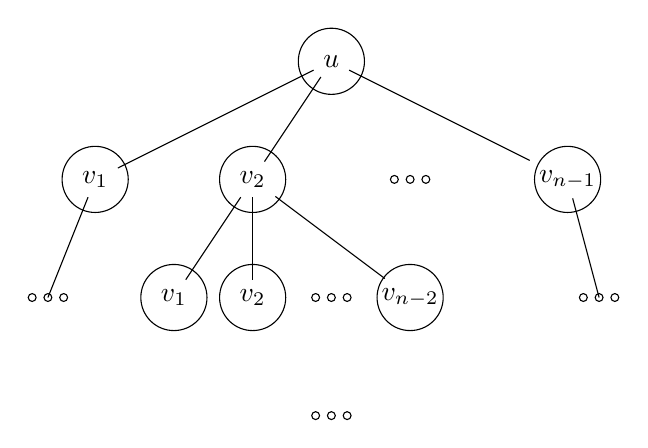
\begin{tikzpicture}
\draw (5, 8) circle [radius=0.42];
\draw (5, 8) node (uno) {$u$};
\draw (2, 6.5) circle [radius=0.42];
\draw (2, 6.5) node (dos) {$v_1$};
\draw (4, 6.5) circle [radius=0.42];
\draw (4, 6.5) node (tres) {$v_2$};
\draw (5.8, 6.5) circle[radius=0.05];
\draw (6.0, 6.5) circle[radius=0.05];
\draw (6.2, 6.5) circle[radius=0.05];
\draw (8, 6.5) circle[radius=0.42];
\draw (8, 6.5) node (cuatro) {$v_{n-1}$};
\draw (uno) -- (dos);
\draw (uno) -- (tres);
\draw (uno) -- (cuatro);
\draw (1.2, 5) circle[radius=0.05];
\draw (1.4, 5) circle[radius=0.05];
\draw (1.6, 5) circle[radius=0.05];
\draw (3, 5) circle[radius=0.42];
\draw (3, 5) node (cinco) {$v_1$};
\draw (4, 5) circle[radius=0.42];
\draw (4, 5) node (seis) {$v_2$};
\draw (4.8, 5) circle[radius=0.05];
\draw (5.0, 5) circle[radius=0.05];
\draw (5.2, 5) circle[radius=0.05];
\draw (6, 5) circle[radius=0.42];
\draw (6, 5) node (siete) {$v_{n-2}$};
\draw (8.2, 5) circle[radius=0.05];
\draw (8.4, 5) circle[radius=0.05];
\draw (8.6, 5) circle[radius=0.05];
\draw (tres) -- (cinco);
\draw (tres) -- (seis);
\draw (tres) -- (siete);
\draw (dos) -- (1.4, 5);
\draw (cuatro) -- (8.4, 5);
\draw (4.8, 3.5) circle[radius=0.05];
\draw (5.0, 3.5) circle[radius=0.05];
\draw (5.2, 3.5) circle[radius=0.05];
\end{tikzpicture}

\caption{\'Arbol de llamadas recursivas. $u$ es el nodo de origen, y $v_i$ es el vecino $i$ disponible para avanzar en la recursi\'on del padre del nodo en el \'arbol}
\label{exacto:arbol_llamadas}
\end{figure}

Si se implementa una \emph{matriz de adyacencia}, obtener los adyacentes se realiza en $O(n)$, con $n$ la cantidad de nodos del grafo.
Marcar un nodo y saber si esta marcado se puede implementar en $O(1)$ con un \emph{array}.
La copia y asignaci\'on de una soluci\'on se puede realizar acot\'andolo por $O(n)$ teniendo un \emph{array} con todos los nodos que tiene el camino, siendo $n$ (total de nodos en el grafo) la cantidad de nodos m\'aximos que puede tener un camino simple.

Se puede plantear una funci\'on de recurrencia para un grafo $K_n$, donde todos los nodos tienen $n - 1$ vecinos, y en cada llamada recursiva se est\'a quitando un vecino posible.
\begin{equation*}
\begin{split}
T(n) = 2n' + (n-1)[T(n-1) + n'] = \\
T(n) = 2n' + (n-1)*T(n-1) + (n-1)*n' = \\
T(n) = (n-1)*T(n-1) + (n+1)*n'
\end{split}
\end{equation*}
Donde $n'$ es igual a la cantidad de nodos siempre, y $n$ representa la a cantidad de nodos disponibles que hay para visitar, inicialmente $n = n'$. Como el grafo es $K_n$, todos los nodos son adyacentes con todos.
El primer $2n'$ que aparece en la equaci\'on representa obtener todos los adyacentes del nodo y el guardar la soluci\'on final cuando se recorri\'o todos los adyacentes, $T(n-1)$ es la llamada recursiva que se realiza $(n-1)$ veces, y el \'ultimo $n'$ es el caso de estar mejorando la soluci\'on y en todas las llamadas tener que copiar siempre la soluci\'on, es decir, copiar $(n-1)$ veces la nueva soluci\'on de tama\~no acotado por $n'$.
\begin{equation*}
\begin{split}
T(n) = (n-1)*T(n-1) + (n+1)*n' \\
= \\
T(n) = (n-1)*[(n-2)*T(n-2) + (n)*n'] + (n+1)*n' \\
= \\
T(n) = (n-1)*(n-2)*T(n-2) + (n-1)*(n)*n'+ (n+1)*n' \\
= \\
T(n) = (n-1)*(n-2)*[(n-3)*T(n-3) + (n-1)*n'] + \\
(n-1)*(n)*n'+ (n+1)*n' \\
= \\
T(n) = (n-1)*(n-2)*(n-3)*T(n-3) + (n-1)^2(n-2)*n' + \\
(n-1)*(n)*n' + (n+1)*n' \\
= \\
T(n) = (n-1)*(n-2)*(n-3)*[(n-4)*T(n-4) + (n-2)*n'] + \\
(n-1)^2*(n-2)*n' + (n-1)*(n)*n' + (n+1)*n' \\
= \\
T(n) = (n-1)*(n-2)*(n-3)*(n-4)*T(n-4) + (n-1)(n-2)^2(n-3)*n' + \\
(n-1)^2*(n-2)*n' + (n-1)*(n)*n' + (n+1)*n' \\
\dots
\end{split}
\end{equation*}
Si se sigue desarrollando la equaci\'on, nos quedar\'ia:
\begin{equation*}
\begin{split}
T(n) = (n - 1)! + n'*\sum_{i=-1}^{n-2}((n-i)\prod_{j=1}^{i+1}(n-j))
\end{split}
\end{equation*}
Como ya no hay recurrencia, y $n = n'$ en la primer llamada, entonces nos queda
\begin{equation*}
\begin{split}
T(n) = (n - 1)! + n*\sum_{i=-1}^{n-2}((n-i)\prod_{j=1}^{i+1}(n-j)) \\
= (n - 1)! + \sum_{i=-1}^{n-2}(n*(n-i)\prod_{j=1}^{i+1}(n-j)) \\
= (n - 1)! + \sum_{i=-1}^{n-2}((n-i)\prod_{j=0}^{i+1}(n-j)) \\
= (n - 1)! + \sum_{i=-1}^{n-2}((n-i)\frac{n!}{(n-i-2)!}) \\
\end{split}
\end{equation*}
Ahora expandimos la suma
\begin{equation*}
\begin{split}
T(n) = (n - 1)! + (n + 1)\frac{n!}{(n-1)!} + (n)\frac{n!}{(n-2)!} + \cdots + 3\frac{n!}{1!} + 2\frac{n!}{0!} \\
\implies T(n) \in O(n!)
\end{split}
\end{equation*}
Quedandonos entonces que la funci\'on de recurrencia que se plante\'o pertenece a la clase de complejidad $O(n!)$

\subsection{Experimentacion: Mediciones de Performance}
En esta secci\'on se mostrar\'an resultados de complejidad temporal emp\'irica, veremos que los resultados coinciden razonablemente con el an\'alisis de complejidad te\'orica..
Para tener una mejor idea del comportamiento del algoritmo, realizamos pruebas sobre grafos aleatorios de distintos tama\~nos(en cantidad de nodos), y por cada cantidad $n$ de nodos, variamos las densidades de aristas dentro de cierto rango alrededor de una funcion de $n$, las densidades elegidas fueron:
\begin{itemize}
	\item m = $a*n + b$. Es decir una cantidad lineal de aristas en base a los nodos. $a \in \mathbb{N}_{>1}$
	\item m = $\frac{n*(n-1)}{2}$. Es decir grafos cercanos o iguales a cliques de n nodos.
\end{itemize}


\textbf{Nota: } Como mencionamos anteriormente, las funciones son variadas en un rango, es decir, por ejemplo, para el caso de cliques, los grafos generados tienen entre $\frac{n*(n-1)}{5}$ y $\frac{n*(n-1)}{2}$ aristas para aleatorizar mas la generacion de grafos densos.\\

\textbf{Nota: } Los graficos que contienen puntos rojos y una curva verde, indican, para cada valor del eje X(cantidad de nodos), los puntos rojos son los tiempos de ejecucion para los diferentes valores de aristas en el rango de la familia, asimismo, la curva verde indica el promedio de estos puntos para cada X. \\

En esta primera secci\'on dividiremos las funciones por polinomios $n$, $n^2$, $n^3$ y $n^4$ con la mayor cantidad de nodos posible e intentaremos ver que la funci\'on se mantiene creciente. Dadas las limitaciones de nuestra computadora de benchmarking, el an\'alisis de divisi\'on por factorial se har\'a aparte con menos cantidad de nodos.

\subsubsection{Rendimiento para grafos con densidad lineal de aristas}

\begin{itemize}
	\item cant nodos min = $10000$
	\item cant nodos max = $12000$
	\item peso maximo w1 = $250$
	\item peso maximo w2 = $400$
	\item step nodos = $500$
	\item step aristas = $1000$
	\item aristas minimas = $(n-1)$
	\item aristas maximas = $(10*n)$
\end{itemize}

\begin{center}
	\textbf{Tiempo de ejecuci\'on en microsegundos para esta familia}\\
	\textbf{$y = f(x)$}\\
	\includegraphics[scale=0.7]{experimentos/resultados_tiempo_exacta_lineales/{exacta.tmpplot_complexity_variation}.png}
\end{center}

\begin{center}
	\textbf{$y = f(x)/x$}\\
	\includegraphics[scale=0.7]{experimentos/resultados_tiempo_exacta_lineales/{exacta.tmpplot_complexity_med_over_n}.png}
\end{center}

\begin{center}
	\textbf{$y = f(x)/x^2$}\\
	\includegraphics[scale=0.7]{experimentos/resultados_tiempo_exacta_lineales/{exacta.tmpplot_complexity_med_over_n_square}.png}
\end{center}

\begin{center}
	\textbf{$y = f(x)/x^3$}\\
	\includegraphics[scale=0.7]{experimentos/resultados_tiempo_exacta_lineales/{exacta.tmpplot_complexity_med_over_n_cube}.png}
\end{center}


\begin{center}
	\textbf{$y = f(x)/x^4$}\\
	\includegraphics[scale=0.7]{experimentos/resultados_tiempo_exacta_lineales/{exacta.tmpplot_complexity_med_over_n_fourth}.png}
\end{center}



\subsubsection{Rendimiento para grafos con densidad cuadratica de aristas}

\begin{itemize}
	\item cant nodos min = $10$
	\item cant nodos max = $600$
	\item peso maximo w1 = $250$
	\item peso maximo w2 = $400$
	\item step nodos = $50$
	\item step aristas = $7000$
	\item aristas minimas = $(n*(n-1))/10$
	\item aristas maximas = $(n*(n-1))/2$
\end{itemize}

\begin{center}
	\textbf{Tiempo de ejecuci\'on en microsegundos para esta familia}\\
	\textbf{$y = f(x)$}\\
	\includegraphics[scale=0.7]{experimentos/resultados_tiempo_exacta_cliques/{exacta.tmpplot_complexity_variation}.png}
\end{center}

\begin{center}
	\textbf{$y = f(x)/x$}\\
	\includegraphics[scale=0.7]{experimentos/resultados_tiempo_exacta_cliques/{exacta.tmpplot_complexity_med_over_n}.png}
\end{center}

\begin{center}
	\textbf{$y = f(x)/x^2$}\\
	\includegraphics[scale=0.7]{experimentos/resultados_tiempo_exacta_cliques/{exacta.tmpplot_complexity_med_over_n_square}.png}
\end{center}

\begin{center}
	\textbf{$y = f(x)/x^3$}\\
	\includegraphics[scale=0.7]{experimentos/resultados_tiempo_exacta_cliques/{exacta.tmpplot_complexity_med_over_n_cube}.png}
\end{center}


\begin{center}
	\textbf{$y = f(x)/x^4$}\\
	\includegraphics[scale=0.7]{experimentos/resultados_tiempo_exacta_cliques/{exacta.tmpplot_complexity_med_over_n_fourth}.png}
\end{center}


En el caso de los grafos con densidad de aristas cuadr\'atica, puede notarse que la curva se sigue manteniendo creciente siendo dividida por todos los polinomios de la experimentaci\'on. Si bien no es concluyente, es un indicio de que la complejidad se sit\'ua en un orden mayor. En los grafos con densidad de aristas lineal, la curva se convierte en constante en el orden cuadr\'atico y decreciente en los siguientes. Suponemos esto se debe a la gran reducc\'on del \'arbol de recursi\'on por la peque\~na cantidad de aristas, la disminuci\'on del grado de los nodos y la calidad de las podas.

\subsubsection{An\'alisis factorial}